\documentclass[a0,landscape]{a0poster}
\pagestyle{empty}
\setcounter{secnumdepth}{0}
\usepackage[absolute]{textpos}
\usepackage{multicol}
\usepackage{subfigure}
\usepackage[pdftex]{graphicx}
\usepackage{graphics}
\usepackage{setspace}
\usepackage{wrapfig,times}
\usepackage{dcolumn}
%\usepackage{booktabs}
\usepackage{ctable}
\usepackage{color}
\definecolor{DarkBlue}{rgb}{0.1,0.1,0.5}
\definecolor{Red}{rgb}{0.9,0.0,0.1}
\usepackage{amsmath}
\usepackage[T1]{fontenc}
\usepackage{fourier}
\usepackage{libertine}
\renewcommand*\oldstylenums[1]{{\fontfamily{fxlj}\selectfont #1}}

% see documentation for a0poster class for the size options here
\let\Textsize\normalsize
\def\Head#1{\noindent{\LARGE\color{DarkBlue} #1}}
\def\LHead#1{\noindent{\Huge\color{DarkBlue} #1}}
\def\Subhead#1{\noindent{\LARGE\color{DarkBlue} #1}\bigskip}
\def\Title#1{\noindent{\VeryHuge\color{Red} #1}}
\def\MHead#1{\noindent{\LARGE\color{Red}#1}\bigskip}


% Set up the grid
%
% Note that [40mm,40mm] is the margin round the edge of the page --
% it is _not_ the grid size. That is always defined as
% PAGE_WIDTH/HGRID and PAGE_HEIGHT/VGRID. In this case we use
% 23 x 12. This gives us three columns of width 7 boxes, with a gap of
% width 1 in between them. 12 vertical boxes is a good number to work
% with.
%
% Note however that texblocks can be positioned fractionally as well,
% so really any convenient grid size can be used.
%
\TPGrid[40mm,40mm]{23}{12}      % 3 cols of width 7, plus 2 gaps width 1

\parindent=0pt
\parskip=0.5\baselineskip

\begin{document}

% Understanding textblocks is the key to being able to do a poster in
% LaTeX. In
%
%    \begin{textblock}{wid}(x,y)
%    ...
%    \end{textblock}
%
% the first argument gives the block width in units of the grid
% cells specified above in \TPGrid; the second gives the (x,y)
% position on the grid, with the y axis pointing down.

% You will have to do a lot of previewing to get everything in the
% right place.

% This gives good title positioning for a portrait poster.
% Watch out for hyphenation in titles - LaTeX will do it
% but it looks awful.
\begin{textblock}{23}(0,0)
\begin{center}
\Title{Excepted Service Appointments and Presidential Unilateral Power}
\end{center}
\end{textblock}

\begin{textblock}{10}(6.5,.75)
\begin{center}
\Huge{Emily H.\ Moore}\\
\LARGE{Department of Political Science}\\
\LARGE{Washington University in St.\ Louis}\\
\end{center}
\end{textblock}

%\begin{textblock}{2}(19.5,.75)
%\begin{center}
%\includegraphics[scale=4]{logo.jpg}
%\end{center}
%\end{textblock}


\begin{textblock}{7}(0,2)
\hrule \bigskip
\Head{Research Question}

\begin{Large}

Where and under what conditions do presidents use Schedule C appointees?

\bigskip
\end{Large}

\hrule \bigskip
\Head{What Are Excepted Appointees?}
\begin{singlespacing}
\begin{Large}
Most people are familiar with the glamour and intrigue of the advice and consent process. However, millions of individuals work for the federal government and only a tiny percentage actually go through advice and consent. 

\smallskip
Excepted appointees are interesting because they are selected by the president but they serve without the Senate's advice and consent. 

\end{Large}
\end{singlespacing}

\bigskip
\bigskip
\hrule
\bigskip

\Head{Motivating Example}

\begin{center}
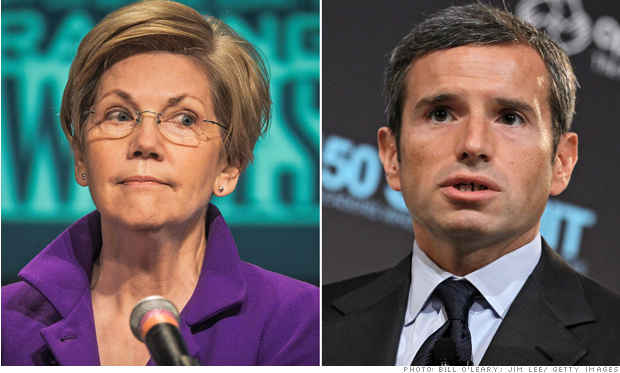
\includegraphics[width=13.2in]{WarrenWeiss.png}
\end{center}
\begin{Large}
In November 2014, President Obama nominated Antonio Weiss as the Undersecretary for Domestic Finance. Led by Elizabeth Warren, a number of progressive Democrats in the Senate opposed Weiss' appointment. To avoid a confirmation showdown, Obama withdrew the nomination and instead appointed Weiss to an excepted position. While he may have fewer formal responsibilities than he would have as Undersecretary, Weiss had the ability to affect policy immediately rather than risking a lengthy and potentially unsuccessful confirmation battle.

\end{Large}

\end{textblock}

\begin{textblock}{7}(8,2)
\hrule \bigskip

\Head{Hypotheses}

\begin{Large}
\begin{itemize}
\item Because presidents need to bolster the work of their allies and will have an easier time influencing agencies sympathetic to their agendas, I expect presidents will utilize Schedule C appointees more frequently in ideologically similar agencies.

\item Given the difficulty that presidents encounter with staffing when there are high levels of congressional polarization, I expect that presidents utilize Schedule C appointees more frequently when Congress is relatively polarized. 
\end{itemize}
\end{Large}

\bigskip
\hrule
\bigskip

\Head{Schedule C Appointees Over Time}

\begin{Large}

The black line in the figure below shows the total number of Schedule C appointees over time. The number of Schedule Cs tends to fall during a presidential transition and then rise as the positions are filled. The purple line is the number of new hires to agencies each year. The number of new hires in 2009 nearly equaled the total number of Schedule Cs in 2009, indicating that over 96 percent of appointees were new hires in the Obama administration rather than holdovers from previous administrations. 

\end{Large}

\begin{center}
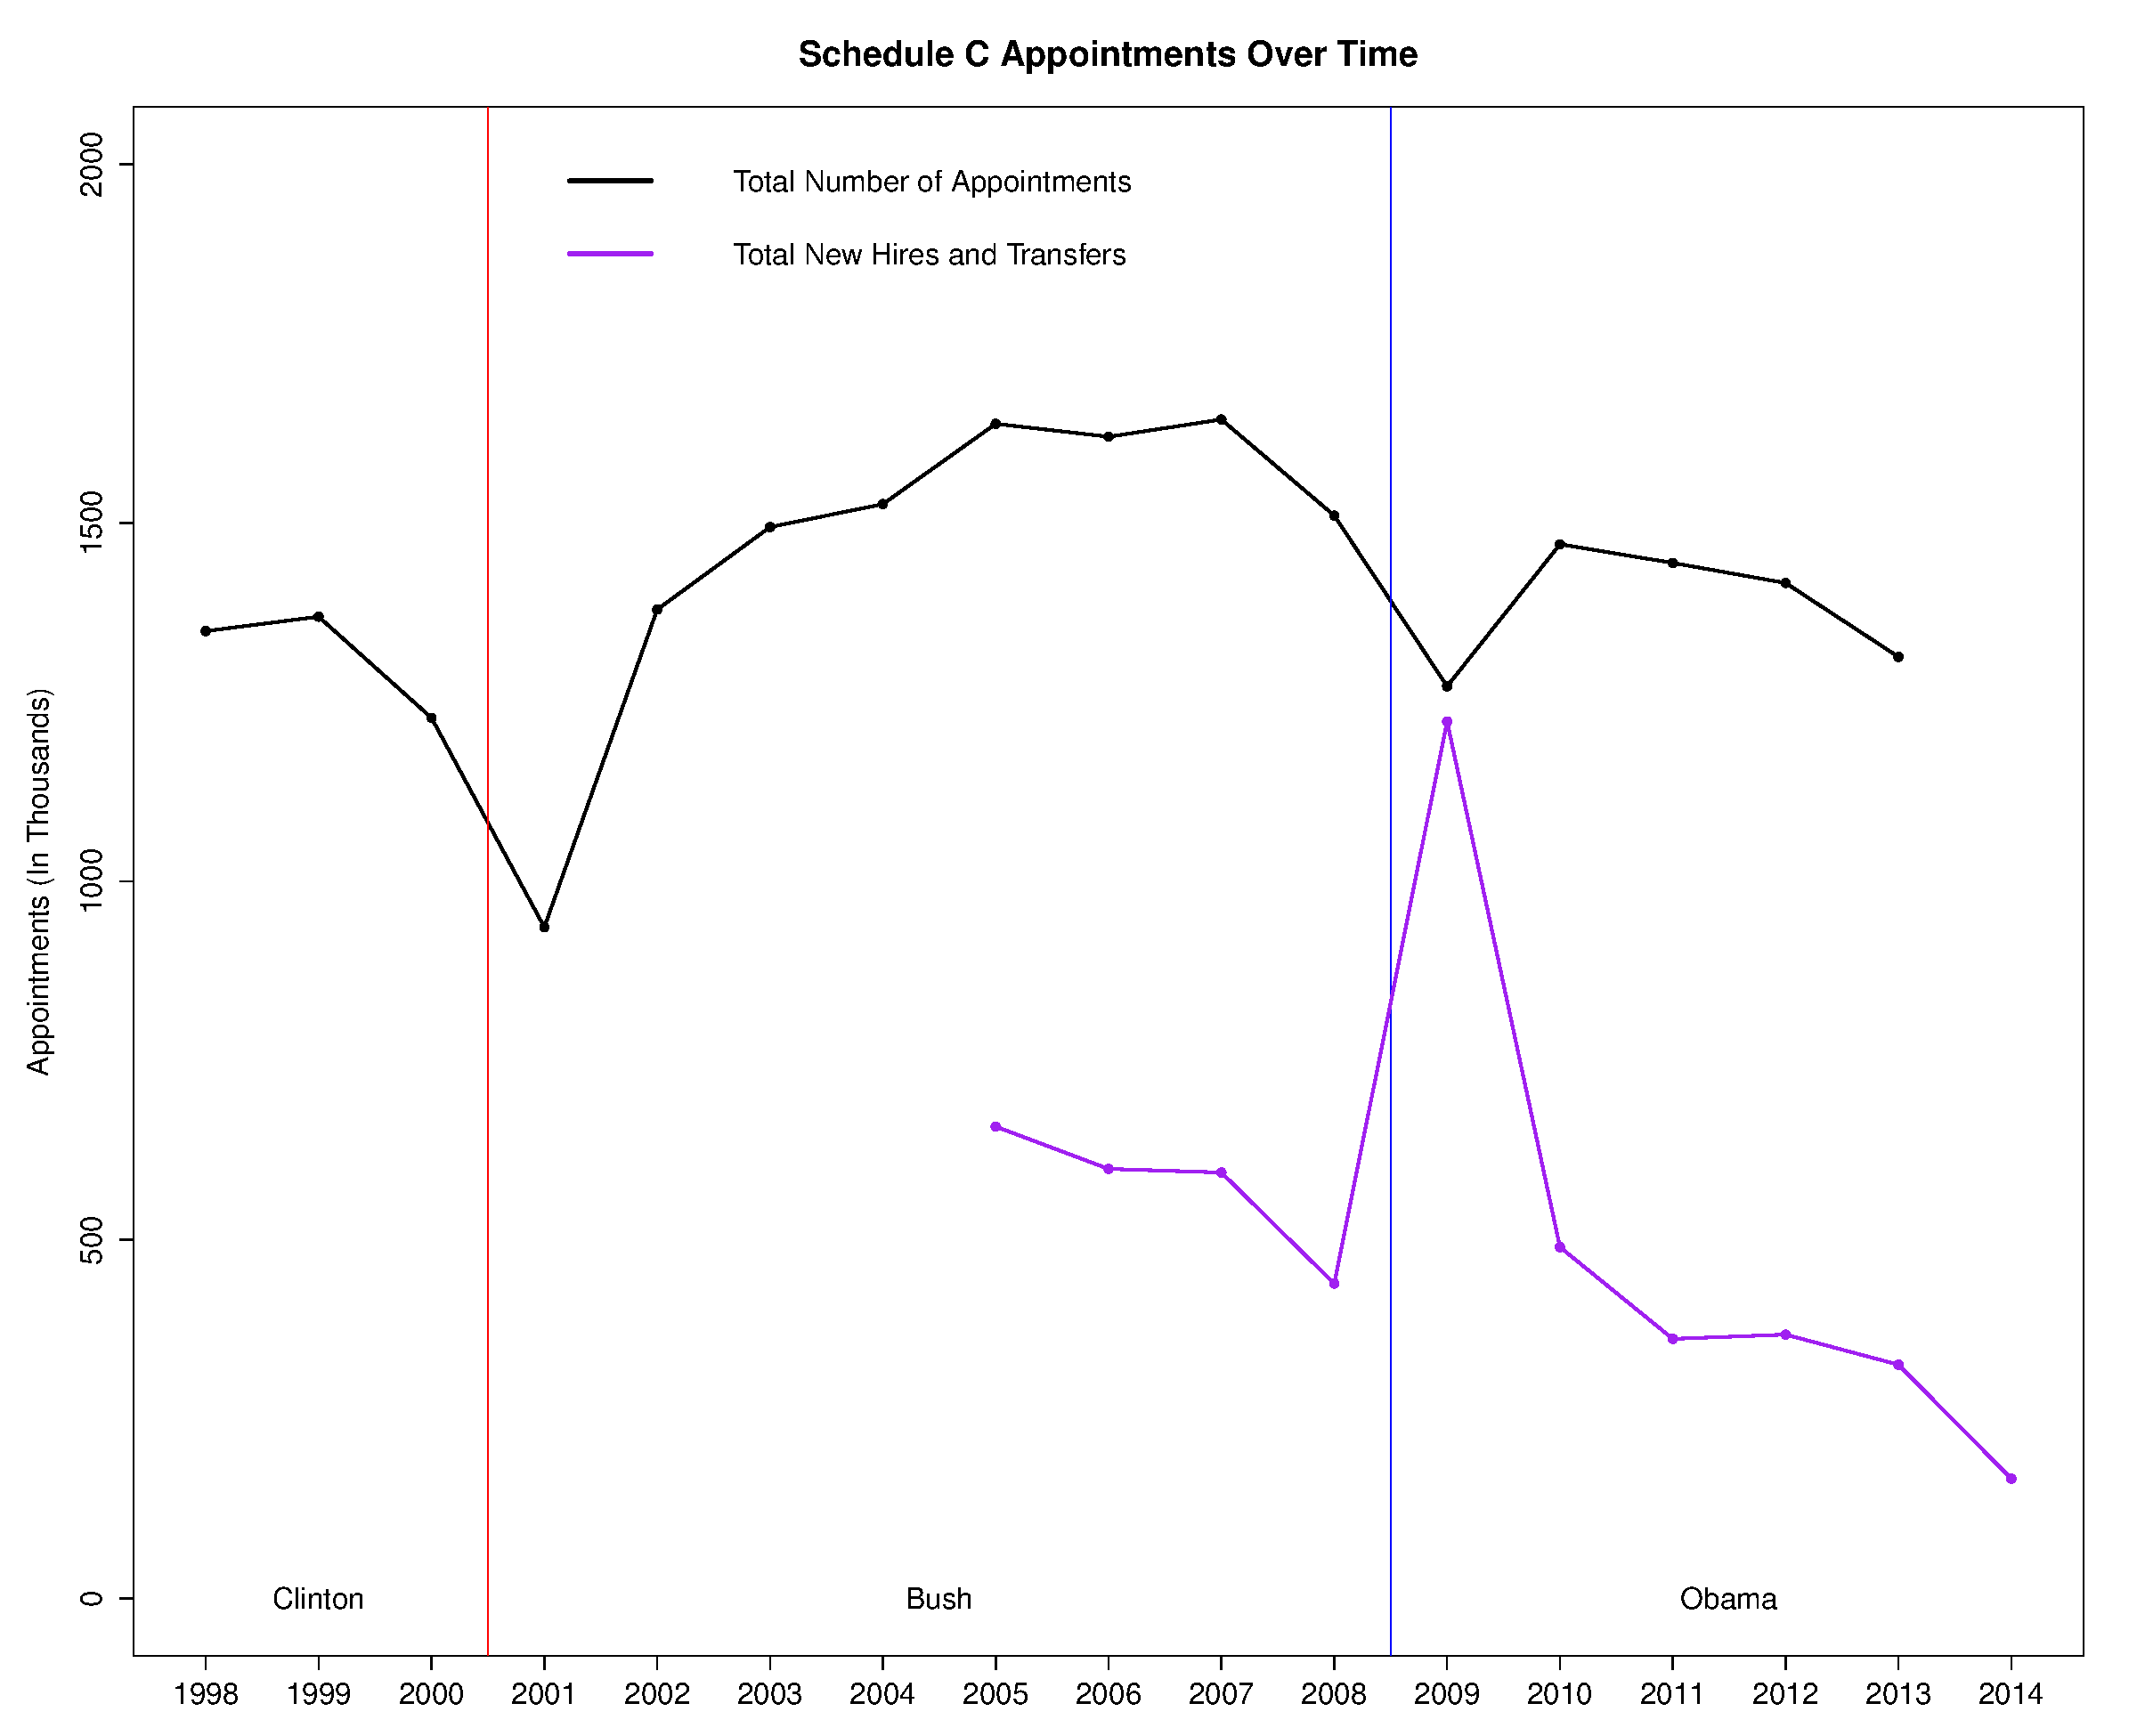
\includegraphics[width=13.2in]{SCAptsandAccOverTime.pdf}
\end{center}

\end{textblock}


\begin{textblock}{7}(16,2)

\hrule \bigskip

\Head{Results}

\bigskip

\begin{Large}

\begin{table}[!htbp] \centering 
Dependent Variable: Number of Schedule Cs
\begin{tabular}{@{\extracolsep{5pt}}lrc} 
\\[-1.8ex]\hline 
\cline{2-3} 
\\[-1.8ex] & \textit{Coefficient} & \textit{Standard Error} \\ 
\hline \\[-1.8ex] 
 Ideological Distance & $-$2.488 & (0.444) \\ 
 Congressional Polarization & 3.070& (0.706) \\ 
 Agency Size & 0.009 & (0.002) \\ 
 First Year of Presidency & $-$0.235 & (0.049) \\ 
 Last Year of Presidency & $-$0.013& (0.023) \\ 
 Obama &  $-$1.516 & (0.277) \\ 
 Clinton  & $-$0.601  & (0.195) \\ 
 Constant & 2.006 & (0.409) \\ 
\hline \\[-1.8ex] 
Observations &  811&\\ 
Log Likelihood & $-$3,209.507 &  \\ 
$\theta$ & 0.451 (0.022) &  \\ 
Akaike Inf. Crit. & 6,435.015 &  \\ 
\hline 
\hline \\[-1.8ex] 
\end{tabular} 

\begin{normalsize}Results are from a Negative Binomial regression model with clustered standard errors.\end{normalsize}
\end{table}  

\end{Large}
\begin{center}
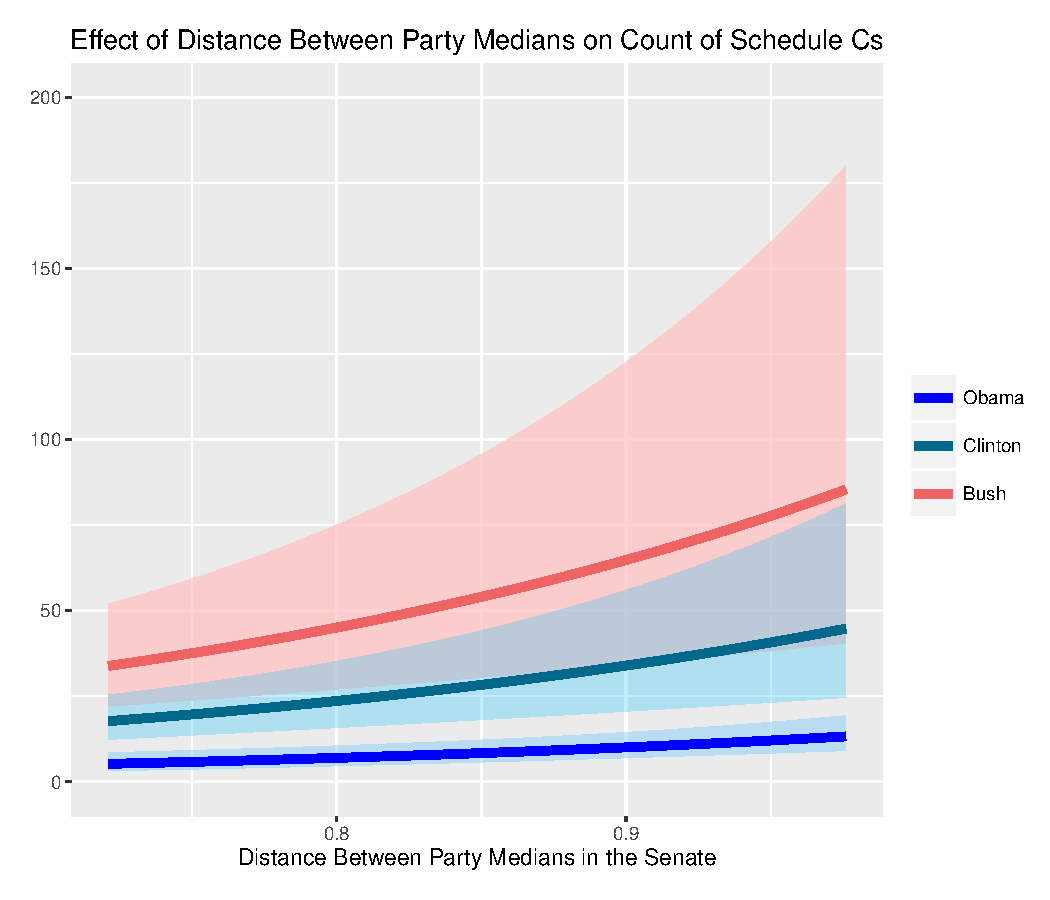
\includegraphics[width=14in]{ResultsPlots.pdf}
\end{center}

\Head{Conclusions}

\begin{Large}
\begin{itemize}
\item Schedule C appointees are a powerful yet understudied tool in the president's unilateral policy arsenal.
\item Evidence suggests presidents utilize Schedule C appointees more frequently in ideologically similar agencies.
\item Evidence also suggests that presidents utilize Schedule C appointees more frequently when conditions in the Senate are unfavorable for confirmations. 
\end{itemize}
\end{Large}

\end{textblock}

\begin{textblock}{23}(0,12.25)
\rule{\textwidth}{.4pt}
\end{textblock}
\end{document}
